% =========================================================
% Algebra of completeness bounds
% =========================================================
\subsection*{Algebraic Properties of Supremum and Infimum}

% =========================================================
% Uniqueness of the Maximum
% =========================================================
\begin{propositionbox}{Proposition (Uniqueness of the Maximum)}
\begin{proposition}[Uniqueness of the Maximum]
\label{prop:uniqueness-of-the-maximum}
Let $A\subseteq\mathbb{R}$. If $m_1$ and $m_2$ are both maximum elements of $A$, then $m_1=m_2$.

\smallskip
\noindent
\hyperref[prf:uniqueness-of-the-maximum]{\textit{Go to proof.}}
\end{proposition}
\end{propositionbox}

\begin{remark*}[Standard quantified statement]
\[
\begin{aligned}
&\text{Let }A\subseteq\mathbb{R}\text{ and }m_1,m_2\in A.\\
&\bigl[m_1\text{ is a maximum of }A
\;\land\;
m_2\text{ is a maximum of }A\bigr]
\Longrightarrow
m_1=m_2.
\end{aligned}
\]
\end{remark*}

\begin{remark*}[Predicate reading]
\[
\operatorname{Maximum}(m_1,A)\land \operatorname{Maximum}(m_2,A)
\Longrightarrow
m_1=m_2.
\]
\end{remark*}

\begin{remark*}[Negated quantified statement]
\[
\begin{aligned}
&\text{Let }A\subseteq\mathbb{R}\text{ and }m_1,m_2\in A.\\
&m_1\text{ and }m_2\text{ are both maximum elements of }A
\text{ and }m_1\ne m_2
\end{aligned}
\]
is impossible.
\end{remark*}

\begin{remark*}[Negation predicate reading]
\[
\operatorname{Maximum}(m_1,A)\land \operatorname{Maximum}(m_2,A)\land m_1\ne m_2
\]
is a contradictory configuration.
\end{remark*}

\begin{remark*}[Failure modes]
The uniqueness claim could fail only if two distinct elements of $A$ each dominated all elements of $A$. In the real order this cannot occur because each maximum must be less than or equal to the other.
\end{remark*}

\begin{remark*}[Failure mode decomposition]
\[
\begin{aligned}
&\operatorname{Maximum}(m_1,A)\land \operatorname{Maximum}(m_2,A)\\
&\qquad\Longrightarrow
\underbrace{m_1\le m_2}_{m_2\text{ dominates }A}
\land
\underbrace{m_2\le m_1}_{m_1\text{ dominates }A}
\Longrightarrow
m_1=m_2.
\end{aligned}
\]
\end{remark*}

\begin{remark*}[Interpretation]
A maximum is not merely a high point of the set; it is the greatest point of the set. If two elements both claim that role, each must sit above the other, and antisymmetry of the real order forces them to be the same number.
\end{remark*}

\begin{remark*}[Dependencies]
\hyperref[def:maximum]{Maximum}.
\end{remark*}


% =========================================================
% Uniqueness of the Supremum
% =========================================================
\begin{propositionbox}{Proposition (Uniqueness of the Supremum)}
\begin{proposition}[Uniqueness of the Supremum]
\label{prop:uniqueness-of-the-supremum}
Let $A\subseteq\mathbb{R}$. If $s_1$ and $s_2$ are both suprema of $A$, then $s_1=s_2$.

\smallskip
\noindent
\hyperref[prf:uniqueness-of-the-supremum]{\textit{Go to proof.}}
\end{proposition}
\end{propositionbox}

\begin{remark*}[Standard quantified statement]
\[
\begin{aligned}
&\text{Let }A\subseteq\mathbb{R}\text{ and }s_1,s_2\in\mathbb{R}.\\
&\bigl[s_1=\sup A\;\land\;s_2=\sup A\bigr]
\Longrightarrow
s_1=s_2.
\end{aligned}
\]
\end{remark*}

\begin{remark*}[Predicate reading]
\[
\operatorname{Supremum}(s_1,A)\land \operatorname{Supremum}(s_2,A)
\Longrightarrow
s_1=s_2.
\]
\end{remark*}

\begin{remark*}[Negated quantified statement]
\[
\begin{aligned}
&\text{Let }A\subseteq\mathbb{R}\text{ and }s_1,s_2\in\mathbb{R}.\\
&s_1=\sup A,\quad s_2=\sup A,\quad\text{and}\quad s_1\ne s_2
\end{aligned}
\]
is impossible.
\end{remark*}

\begin{remark*}[Negation predicate reading]
\[
\operatorname{Supremum}(s_1,A)\land \operatorname{Supremum}(s_2,A)\land s_1\ne s_2
\]
is a contradictory configuration.
\end{remark*}

\begin{remark*}[Failure modes]
The uniqueness claim could fail only if two different real numbers were both least upper bounds of the same set. Since each supremum is less than or equal to every upper bound, each must be less than or equal to the other.
\end{remark*}

\begin{remark*}[Failure mode decomposition]
\[
\begin{aligned}
&\operatorname{Supremum}(s_1,A)\land \operatorname{Supremum}(s_2,A)\\
&\qquad\Longrightarrow
\underbrace{s_1\le s_2}_{s_2\text{ is an upper bound and }s_1\text{ is least}}
\land
\underbrace{s_2\le s_1}_{s_1\text{ is an upper bound and }s_2\text{ is least}}
\Longrightarrow
s_1=s_2.
\end{aligned}
\]
\end{remark*}

\begin{remark*}[Interpretation]
The supremum is the least possible ceiling over a set. Two ceilings can both be least only if neither one is actually above the other, so the order on $\mathbb{R}$ identifies them as the same number.
\end{remark*}

\begin{remark*}[Dependencies]
\hyperref[def:supremum]{Supremum}.
\end{remark*}


% =========================================================
% Maximum Implies Supremum
% =========================================================
\begin{propositionbox}{Proposition (Maximum Implies Supremum)}
\begin{proposition}[Maximum Implies Supremum]
\label{prop:maximum-implies-supremum}
Let $A\subseteq\mathbb{R}$ and let $m\in A$. If $m$ is a maximum of $A$, then $m=\sup A$.

\smallskip
\noindent
\hyperref[prf:maximum-implies-supremum]{\textit{Go to proof.}}
\end{proposition}
\end{propositionbox}

\begin{remark*}[Standard quantified statement]
\[
\begin{aligned}
&\text{Let }A\subseteq\mathbb{R}\text{ and }m\in A.\\
&m\text{ is a maximum of }A
\Longrightarrow
m=\sup A.
\end{aligned}
\]
\end{remark*}

\begin{remark*}[Predicate reading]
\[
\operatorname{Maximum}(m,A)
\Longrightarrow
\operatorname{Supremum}(m,A).
\]
\end{remark*}

\begin{remark*}[Negated quantified statement]
\[
\begin{aligned}
&\text{Let }A\subseteq\mathbb{R}\text{ and }m\in A.\\
&m\text{ is a maximum of }A
\text{ and }m\ne\sup A
\end{aligned}
\]
is impossible.
\end{remark*}

\begin{remark*}[Negation predicate reading]
\[
\operatorname{Maximum}(m,A)\land \neg\operatorname{Supremum}(m,A)
\]
is a contradictory configuration.
\end{remark*}

\begin{remark*}[Failure modes]
The implication could fail only if the greatest element of $A$ were not the least upper bound of $A$. But a maximum already bounds the set from above, and every upper bound must lie at least as high as that maximum.
\end{remark*}

\begin{remark*}[Failure mode decomposition]
\[
\begin{aligned}
\operatorname{Maximum}(m,A)
&\Longrightarrow
\underbrace{\forall x\in A\;(x\le m)}_{m\text{ is an upper bound}}\\
&\qquad\land
\underbrace{\forall u\in\mathbb{R}\,
\bigl[(\forall x\in A\;(x\le u))\Longrightarrow m\le u\bigr]}_{m\text{ is least among upper bounds}}.
\end{aligned}
\]
\end{remark*}

\begin{remark*}[Interpretation]
A maximum belongs to the set and sits above every element of the set. That makes it an upper bound, and no smaller upper bound can exist because it would have to sit below the maximum while still bounding the maximum itself.
\end{remark*}

\begin{remark*}[Dependencies]
\hyperref[def:maximum]{Maximum};
\hyperref[def:supremum]{Supremum}.
\end{remark*}


% =========================================================
% Supremum in the Set Is the Maximum
% =========================================================
\begin{propositionbox}{Proposition (Supremum in the Set Is the Maximum)}
\begin{proposition}[Supremum in the Set Is the Maximum]
\label{prop:supremum-in-the-set-is-the-maximum}
Let $A\subseteq\mathbb{R}$ and let $s=\sup A$. If $s\in A$, then $s$ is a maximum of $A$.

\smallskip
\noindent
\hyperref[prf:supremum-in-the-set-is-the-maximum]{\textit{Go to proof.}}
\end{proposition}
\end{propositionbox}

\begin{remark*}[Standard quantified statement]
\[
\begin{aligned}
&\text{Let }A\subseteq\mathbb{R}\text{ and }s\in\mathbb{R}.\\
&\bigl[s=\sup A\;\land\;s\in A\bigr]
\Longrightarrow
s\text{ is a maximum of }A.
\end{aligned}
\]
\end{remark*}

\begin{remark*}[Predicate reading]
\[
\operatorname{Supremum}(s,A)\land s\in A
\Longrightarrow
\operatorname{Maximum}(s,A).
\]
\end{remark*}

\begin{remark*}[Negated quantified statement]
\[
\begin{aligned}
&\text{Let }A\subseteq\mathbb{R}\text{ and }s\in\mathbb{R}.\\
&s=\sup A,\quad s\in A,\quad\text{and }s\text{ is not a maximum of }A
\end{aligned}
\]
is impossible.
\end{remark*}

\begin{remark*}[Negation predicate reading]
\[
\operatorname{Supremum}(s,A)\land s\in A\land \neg\operatorname{Maximum}(s,A)
\]
is a contradictory configuration.
\end{remark*}

\begin{remark*}[Failure modes]
The implication could fail only if the least upper bound belonged to the set but did not dominate every element of the set. That cannot happen because every supremum is already an upper bound.
\end{remark*}

\begin{remark*}[Failure mode decomposition]
\[
\begin{aligned}
\operatorname{Supremum}(s,A)\land s\in A
&\Longrightarrow
\underbrace{\forall x\in A\;(x\le s)}_{s\text{ is an upper bound}}\\
&\qquad\land
\underbrace{s\in A}_{s\text{ belongs to the set}}
\Longrightarrow
\operatorname{Maximum}(s,A).
\end{aligned}
\]
\end{remark*}

\begin{remark*}[Interpretation]
A supremum is usually only a least ceiling. When that ceiling is actually a member of the set, it becomes the greatest element of the set, so the extremal value is attained rather than merely approached.
\end{remark*}

\begin{remark*}[Dependencies]
\hyperref[def:supremum]{Supremum};
\hyperref[def:maximum]{Maximum}.
\end{remark*}




% volume-iii/bounding/figure-supremum-algebra.tex
% TikZ Code only, per House Constitution Rule 2.6
\usetikzlibrary{shapes, positioning, calc, math, decorations.pathreplacing, patterns}

\begin{figure}H]
\centering
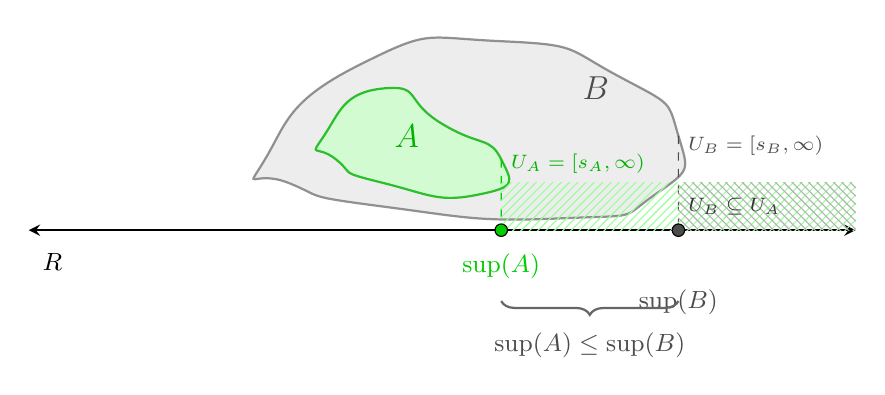
\begin{tikzpicture}[scale=1.5]

    % =========================================================
    % 1. Shared Real Number Line (Ambient Environment, R11.2)
    % =========================================================
    \draw[thick, <->, >=stealth] (-1, 0) -- (6, 0);
    \node[below=5pt, font=\small] at (-0.8, 0) {$\mathbb{R}$};

    % =========================================================
    % 2. Set Definition (Geometric Picture, R7.4)
    % =========================================================

    % Set B (Gray/Outer Blob, Neutral support, R13.4)
    \path[draw, black!60!white, fill=black!10!white, thick, opacity=0.7,
          smooth cycle, tension=1.1] 
        plot coordinates {(1, 0.6) (1.8, 1.4) (3, 1.6) (4, 1.3) (4.5, 0.8) (4.3, 0.3) (3.5, 0.1) (2, 0.2) (1.2, 0.4)};
    \node[black!70!white, font=\large\bfseries] at (3.8, 1.2) {$B$};

    % Set A (Green/Inner Blob)
    \path[draw, green!70!black, fill=green!20!white, thick, opacity=0.8,
          smooth cycle, tension=1.2] 
        plot coordinates {(1.5, 0.8) (2, 1.2) (2.5, 0.9) (3, 0.6) (2.8, 0.3) (2, 0.4) (1.6, 0.6)};
    \node[green!70!black, font=\large\bfseries] at (2.2, 0.8) {$A$};

    % =========================================================
    % 3. Arithmetic Projections (Point-Based Dimension, R7.1)
    % =========================================================

    % Define rightmost (supremal) points for projections
    \coordinate (sup_A_pt) at (3.0, 0.6); 
    \coordinate (sup_B_pt) at (4.5, 0.8); 

    % Draw projections from blobs down to the number line
    \draw[green!80!black, dashed] (sup_A_pt) -- (3.0, 0);
    \draw[black!70!white, dashed] (sup_B_pt) -- (4.5, 0);

    % =========================================================
    % 4. Guard Territory / Upper Bounds (Logical Form Structure, R10.2)
    % =========================================================

    % Shaded Region 1: Territory of Upper Bounds for A (U_A)
    \fill[pattern=north east lines, pattern color=green!40!white] (3.0, 0) rectangle (6, 0.4);

    % Shaded Region 2: Territory of Upper Bounds for B (U_B)
    \fill[pattern=north west lines, pattern color=black!30!white] (4.5, 0) rectangle (6, 0.4);

    % =========================================================
    % 5. Labels and Constraints (Canonical Logic, R7.1, R7.4)
    % =========================================================

    % Mark s_A = sup A on number line
    \draw[fill=green!80!black] (3.0, 0) circle (1.5pt);
    \node[below=5pt, green!80!black, font=\small] (label_supA) at (3.0, 0) {$\sup(A)$};

    % Mark s_B = sup B on number line
    \draw[fill=black!70!white] (4.5, 0) circle (1.5pt);
    \node[below=18pt, black!70!white, font=\small] (label_supB) at (4.5, 0) {$\sup(B)$};

    % Logical Labels in Territory (Relocated to avoid overlap)
    \node[above right, font=\scriptsize, green!70!black] at (3.0, 0.4) {$U_A = [s_A, \infty)$};
    \node[above right, font=\scriptsize, black!70!white] at (4.5, 0.55) {$U_B = [s_B, \infty)$};
    \node[right, font=\scriptsize, black!80] at (4.5, 0.2) {$U_B \subseteq U_A$};

    % =========================================================
    % 6. The Conclusion / The Result (R7.4)
    % =========================================================

    % Visualize the monotonicity inequality: s_A <= s_B
    \draw[decorate, decoration={brace, amplitude=5pt, mirror}, thick, black!60!white] 
        (3.0, -0.6) -- (4.5, -0.6);
    \node[below=8pt, black!70!white, font=\small] at (3.75, -0.6) {
        $\sup(A) \le \sup(B)$
    };

\end{tikzpicture}

\smallskip
\noindent
\textbf{Caption (R7.5, R13.8):} 
Figure \ref{fig:supremum-algebra}: The Monotonicity of Supremum Under Set Inclusion.
This visualization illustrates the arithmetic consequence of set inclusion, $A \subseteq B \subset \mathbb{R}$. The topology of the sets is represented by nested blobs where $A$ (green) is contained within $B$ (gray). Vertically dashed projections link the supremal boundary of each set down to the shared real axis, defining the unique points $s_A = \sup(A)$ and $s_B = \sup(B)$. The figure demonstrates that because the territory of $A$ is restricted by $B$, its maximum guard point $s_A$ cannot exceed $s_B$. Finally, the shaded regions illustrate the territories of upper bounds ($U_A$ and $U_B$), clearly showing that $U_B$ is a proper subset of $U_A$. Any value guarding the larger set $B$ necessarily satisfies the guard condition for the smaller set $A$.
\label{fig:supremum-algebra}
\end{figure}



% =========================================================
% Subset Inclusion Preserves Upper Bounds
% =========================================================
\begin{lemmabox}{Lemma (Subset Inclusion Preserves Upper Bounds)}
\begin{lemma}[Subset Inclusion Preserves Upper Bounds]
\label{lem:subset-inclusion-preserves-upper-bounds}
Let $A\subseteq B\subseteq\mathbb{R}$. If $u$ is an upper bound of $B$, then $u$ is an upper bound of $A$.

\smallskip
\noindent
\hyperref[prf:subset-inclusion-preserves-upper-bounds]{\textit{Go to proof.}}
\end{lemma}
\end{lemmabox}

\begin{remark*}[Standard quantified statement]
\[
\begin{aligned}
&\text{Let }A\subseteq B\subseteq\mathbb{R}\text{ and }u\in\mathbb{R}.\\
&\bigl[\forall y\in B\;(y\le u)\bigr]
\Longrightarrow
\bigl[\forall x\in A\;(x\le u)\bigr].
\end{aligned}
\]
\end{remark*}

\begin{remark*}[Predicate reading]
\[
A\subseteq B\land \operatorname{UpperBound}(u,B)
\Longrightarrow
\operatorname{UpperBound}(u,A).
\]
\end{remark*}

\begin{remark*}[Negated quantified statement]
\[
\begin{aligned}
&A\subseteq B,\quad u\text{ is an upper bound of }B,\\
&\text{and }u\text{ is not an upper bound of }A
\end{aligned}
\]
is impossible.
\end{remark*}

\begin{remark*}[Negation predicate reading]
\[
A\subseteq B\land \operatorname{UpperBound}(u,B)\land \neg\operatorname{UpperBound}(u,A)
\]
is a contradictory configuration.
\end{remark*}

\begin{remark*}[Failure modes]
The implication could fail only if some $x\in A$ exceeded $u$. Since $A\subseteq B$, that same $x$ would belong to $B$, contradicting that $u$ bounds $B$ from above.
\end{remark*}

\begin{remark*}[Failure mode decomposition]
\[
\begin{aligned}
\neg\operatorname{UpperBound}(u,A)
&\Longleftrightarrow
\underbrace{\exists x\in A\;(u<x)}_{\text{witness in }A}\\
&\Longrightarrow
\underbrace{\exists x\in B\;(u<x)}_{A\subseteq B}
\Longleftrightarrow
\neg\operatorname{UpperBound}(u,B).
\end{aligned}
\]
\end{remark*}

\begin{remark*}[Interpretation]
A bound for a larger set automatically bounds every smaller set inside it. Inclusion can only remove possible counterexamples, so it cannot destroy an existing upper bound.
\end{remark*}

\begin{remark*}[Dependencies]
\hyperref[def:upper-bound]{Upper Bound}.
\end{remark*}


% =========================================================
% Supremum Is Monotone Under Inclusion
% =========================================================
\begin{theorembox}{Theorem (Supremum Is Monotone Under Inclusion)}
\begin{theorem}[Supremum Is Monotone Under Inclusion]
\label{thm:supremum-is-monotone-under-inclusion}
Let $A,B\subseteq\mathbb{R}$ be nonempty sets that are bounded above. If $A\subseteq B$, then $\sup A\le \sup B$.

\smallskip
\noindent
\hyperref[prf:supremum-is-monotone-under-inclusion]{\textit{Go to proof.}}
\end{theorem}
\end{theorembox}

\begin{remark*}[Standard quantified statement]
\[
\begin{aligned}
&\text{Let }A,B\subseteq\mathbb{R}\text{ be nonempty and bounded above.}\\
&A\subseteq B
\Longrightarrow
\sup A\le \sup B.
\end{aligned}
\]
\end{remark*}

\begin{remark*}[Predicate reading]
\[
A\subseteq B\land \operatorname{Supremum}(s_A,A)\land \operatorname{Supremum}(s_B,B)
\Longrightarrow
s_A\le s_B.
\]
\end{remark*}

\begin{remark*}[Negated quantified statement]
\[
A\subseteq B,\quad \sup B<\sup A
\]
is impossible when $A$ and $B$ are nonempty and bounded above.
\end{remark*}

\begin{remark*}[Negation predicate reading]
\[
A\subseteq B\land \operatorname{Supremum}(s_A,A)\land \operatorname{Supremum}(s_B,B)\land s_B<s_A
\]
is a contradictory configuration.
\end{remark*}

\begin{remark*}[Failure modes]
The monotonicity statement could fail only if the larger set had a strictly smaller least upper bound. But every upper bound for $B$ is also an upper bound for $A$, so the least upper bound of $A$ cannot sit above $\sup B$.
\end{remark*}

\begin{remark*}[Failure mode decomposition]
\[
\begin{aligned}
A\subseteq B
&\Longrightarrow
\underbrace{\operatorname{UpperBound}(\sup B,A)}_{\sup B\text{ bounds the smaller set}}\\
&\Longrightarrow
\underbrace{\sup A\le \sup B}_{\sup A\text{ is least among upper bounds of }A}.
\end{aligned}
\]
\end{remark*}

\begin{remark*}[Interpretation]
Making a set larger can only push its least ceiling upward or leave it unchanged. It cannot lower the supremum, because the larger set contains all of the old points that already had to be bounded.
\end{remark*}

\begin{remark*}[Dependencies]
\hyperref[def:upper-bound]{Upper Bound};
\hyperref[def:supremum]{Supremum};
\hyperref[lem:subset-inclusion-preserves-upper-bounds]{Subset Inclusion Preserves Upper Bounds}.
\end{remark*}


% =========================================================
% Upper Bound Comparison with the Supremum
% =========================================================
\begin{propositionbox}{Proposition (Upper Bound Comparison with the Supremum)}
\begin{proposition}[Upper Bound Comparison with the Supremum]
\label{prop:upper-bound-comparison-with-the-supremum}
Let $A\subseteq\mathbb{R}$ be nonempty and bounded above, and let $s=\sup A$. For $u\in\mathbb{R}$, the number $u$ is an upper bound of $A$ if and only if $s\le u$.

\smallskip
\noindent
\hyperref[prf:upper-bound-comparison-with-the-supremum]{\textit{Go to proof.}}
\end{proposition}
\end{propositionbox}

\begin{remark*}[Standard quantified statement]
\[
\begin{aligned}
&\text{Let }A\subseteq\mathbb{R}\text{ be nonempty and bounded above, and let }s=\sup A.\\
&\forall u\in\mathbb{R}\;
\bigl[u\text{ is an upper bound of }A
\Longleftrightarrow
s\le u\bigr].
\end{aligned}
\]
\end{remark*}

\begin{remark*}[Predicate reading]
\[
\operatorname{Supremum}(s,A)
\Longrightarrow
\forall u\in\mathbb{R}\;
\bigl[\operatorname{UpperBound}(u,A)\Longleftrightarrow s\le u\bigr].
\]
\end{remark*}

\begin{remark*}[Negated quantified statement]
\[
\exists u\in\mathbb{R}\;
\bigl[
(u\text{ is an upper bound of }A\text{ and }u<s)
\;\lor\;
(s\le u\text{ and }u\text{ is not an upper bound of }A)
\bigr]
\]
is impossible when $s=\sup A$.
\end{remark*}

\begin{remark*}[Negation predicate reading]
\[
\operatorname{Supremum}(s,A)\land
\exists u\in\mathbb{R}\;
\bigl[
(\operatorname{UpperBound}(u,A)\land u<s)
\lor
(s\le u\land \neg\operatorname{UpperBound}(u,A))
\bigr]
\]
is a contradictory configuration.
\end{remark*}

\begin{remark*}[Failure modes]
There are two apparent ways the equivalence could fail. Either an upper bound lies below the supremum, contradicting leastness, or a number above the supremum fails to bound the set, contradicting that the supremum already bounds the set.
\end{remark*}

\begin{remark*}[Failure mode decomposition]
\[
\begin{aligned}
\operatorname{UpperBound}(u,A)&\Longrightarrow s\le u,\\
s\le u&\Longrightarrow
\underbrace{\forall x\in A\;(x\le s)}_{s\text{ bounds }A}
\Longrightarrow
\underbrace{\forall x\in A\;(x\le u)}_{u\text{ also bounds }A}.
\end{aligned}
\]
\end{remark*}

\begin{remark*}[Interpretation]
Once the supremum is known, all upper bounds are exactly the real numbers at or above it. The supremum is therefore the threshold where upper bounds begin.
\end{remark*}

\begin{remark*}[Dependencies]
\hyperref[def:upper-bound]{Upper Bound};
\hyperref[def:supremum]{Supremum}.
\end{remark*}


% =========================================================
% Every Element Lies Below the Supremum
% =========================================================
\begin{propositionbox}{Proposition (Every Element Lies Below the Supremum)}
\begin{proposition}[Every Element Lies Below the Supremum]
\label{prop:every-element-lies-below-the-supremum}
Let $A\subseteq\mathbb{R}$ be nonempty and bounded above, and let $s=\sup A$. Then $x\le s$ for every $x\in A$.

\smallskip
\noindent
\hyperref[prf:every-element-lies-below-the-supremum]{\textit{Go to proof.}}
\end{proposition}
\end{propositionbox}

\begin{remark*}[Standard quantified statement]
\[
\begin{aligned}
&\text{Let }A\subseteq\mathbb{R}\text{ be nonempty and bounded above, and let }s=\sup A.\\
&\forall x\in A\;(x\le s).
\end{aligned}
\]
\end{remark*}

\begin{remark*}[Predicate reading]
\[
\operatorname{Supremum}(s,A)
\Longrightarrow
\forall x\in A\;(x\le s).
\]
\end{remark*}

\begin{remark*}[Negated quantified statement]
\[
s=\sup A\quad\text{and}\quad \exists x\in A\;(s<x)
\]
is impossible.
\end{remark*}

\begin{remark*}[Negation predicate reading]
\[
\operatorname{Supremum}(s,A)\land \exists x\in A\;(s<x)
\]
is a contradictory configuration.
\end{remark*}

\begin{remark*}[Failure modes]
The statement could fail only if some element of $A$ sat strictly above $\sup A$. That would mean $\sup A$ is not even an upper bound of $A$.
\end{remark*}

\begin{remark*}[Failure mode decomposition]
\[
\neg\bigl[\forall x\in A\;(x\le s)\bigr]
\Longleftrightarrow
\underbrace{\exists x\in A\;(s<x)}_{\text{element above the alleged supremum}}
\Longleftrightarrow
\neg\operatorname{UpperBound}(s,A).
\]
\end{remark*}

\begin{remark*}[Interpretation]
The supremum is a ceiling for the set. It may or may not be a point of the set, but every actual element of the set must lie at or below it.
\end{remark*}

\begin{remark*}[Dependencies]
\hyperref[def:upper-bound]{Upper Bound};
\hyperref[def:supremum]{Supremum}.
\end{remark*}


% =========================================================
% Infimum Is Less Than or Equal to the Supremum
% =========================================================
\begin{theorembox}{Theorem (Infimum Is Less Than or Equal to the Supremum)}
\begin{theorem}[Infimum Is Less Than or Equal to the Supremum]
\label{thm:infimum-less-than-supremum}
Let $A\subseteq\mathbb{R}$ be nonempty, bounded below, and bounded above. Then $\inf A\le \sup A$.

\smallskip
\noindent
\hyperref[prf:infimum-less-than-supremum]{\textit{Go to proof.}}
\end{theorem}
\end{theorembox}

\begin{remark*}[Standard quantified statement]
\[
\begin{aligned}
&\text{Let }A\subseteq\mathbb{R}\text{ be nonempty, bounded below, and bounded above.}\\
&\inf A\le \sup A.
\end{aligned}
\]
\end{remark*}

\begin{remark*}[Predicate reading]
\[
\operatorname{Infimum}(t,A)\land \operatorname{Supremum}(s,A)
\Longrightarrow
t\le s.
\]
\end{remark*}

\begin{remark*}[Negated quantified statement]
\[
\inf A>\sup A
\]
is impossible for a nonempty set that has both bounds.
\end{remark*}

\begin{remark*}[Negation predicate reading]
\[
\operatorname{Infimum}(t,A)\land \operatorname{Supremum}(s,A)\land s<t
\]
is a contradictory configuration.
\end{remark*}

\begin{remark*}[Failure modes]
The inequality could fail only if the greatest lower bound were strictly above the least upper bound. Any element of the nonempty set must lie between those two bounding values, which rules out this order.
\end{remark*}

\begin{remark*}[Failure mode decomposition]
\[
\begin{aligned}
&\text{Choose }a\in A.\\
&\underbrace{\inf A\le a}_{\inf A\text{ is a lower bound threshold}}
\quad\text{and}\quad
\underbrace{a\le \sup A}_{\sup A\text{ is an upper bound threshold}}
\Longrightarrow
\inf A\le \sup A.
\end{aligned}
\]
\end{remark*}

\begin{remark*}[Interpretation]
A nonempty bounded set cannot have its floor above its ceiling. Any point of the set witnesses the bridge from the infimum up to the supremum.
\end{remark*}

\begin{remark*}[Dependencies]
\hyperref[def:infimum]{Infimum};
\hyperref[def:supremum]{Supremum}.
\end{remark*}


% =========================================================
% Order Comparison of Suprema
% =========================================================
\begin{propositionbox}{Proposition (Order Comparison of Suprema)}
\begin{proposition}[Order Comparison of Suprema]
\label{prop:order-comparison-of-suprema}
Let $A,B\subseteq\mathbb{R}$ be nonempty and bounded above. If for every $x\in A$ there exists $y\in B$ such that $x\le y$, then $\sup A\le \sup B$.

\smallskip
\noindent
\hyperref[prf:order-comparison-of-suprema]{\textit{Go to proof.}}
\end{proposition}
\end{propositionbox}

\begin{remark*}[Standard quantified statement]
\[
\begin{aligned}
&\text{Let }A,B\subseteq\mathbb{R}\text{ be nonempty and bounded above.}\\
&\bigl[\forall x\in A\;\exists y\in B\;(x\le y)\bigr]
\Longrightarrow
\sup A\le \sup B.
\end{aligned}
\]
\end{remark*}

\begin{remark*}[Predicate reading]
\[
\bigl[\forall x\in A\;\exists y\in B\;(x\le y)\bigr]
\land
\operatorname{Supremum}(s_A,A)\land \operatorname{Supremum}(s_B,B)
\Longrightarrow
s_A\le s_B.
\]
\end{remark*}

\begin{remark*}[Negated quantified statement]
\[
\bigl[\forall x\in A\;\exists y\in B\;(x\le y)\bigr]
\quad\text{and}\quad
\sup B<\sup A
\]
is impossible.
\end{remark*}

\begin{remark*}[Negation predicate reading]
\[
\bigl[\forall x\in A\;\exists y\in B\;(x\le y)\bigr]
\land
\operatorname{Supremum}(s_A,A)\land \operatorname{Supremum}(s_B,B)\land s_B<s_A
\]
is a contradictory configuration.
\end{remark*}

\begin{remark*}[Failure modes]
The comparison could fail only if the supremum of $A$ rose above the supremum of $B$. But every element of $A$ is dominated by some element of $B$, and every element of $B$ lies below $\sup B$, so $\sup B$ is an upper bound for $A$.
\end{remark*}

\begin{remark*}[Failure mode decomposition]
\[
\begin{aligned}
\forall x\in A\;\exists y\in B\;(x\le y)
&\Longrightarrow
\underbrace{\forall x\in A\;(x\le \sup B)}_{\sup B\text{ bounds }A}\\
&\Longrightarrow
\underbrace{\sup A\le \sup B}_{\sup A\text{ is least among upper bounds of }A}.
\end{aligned}
\]
\end{remark*}

\begin{remark*}[Interpretation]
This criterion compares two sets without requiring inclusion. If every point of $A$ can be matched below some point of $B$, then $B$ reaches at least as high as $A$ in the supremum sense.
\end{remark*}

\begin{remark*}[Dependencies]
\hyperref[def:supremum]{Supremum};
\hyperref[prop:every-element-lies-below-the-supremum]{Every Element Lies Below the Supremum};
\hyperref[prop:upper-bound-comparison-with-the-supremum]{Upper Bound Comparison with the Supremum}.
\end{remark*}





% --- Algebra of Supremum Cluster ---

\begin{theorembox}{Theorem (Translation Invariance of the Supremum)}
\begin{theorem}[Translation Invariance of the Supremum]
\label{thm:translation-invariance-supremum}
Let $A\subseteq\mathbb{R}$ be nonempty and bounded above, and let $c\in\mathbb{R}$. Then
\[
  \sup(A+c)=\sup A+c,
  \qquad
  A+c=\{a+c:a\in A\}.
\]
\hyperref[prf:translation-invariance-supremum]{Go to proof.}
\end{theorem}
\end{theorembox}

\begin{remark*}[Standard quantified statement]
\[
\begin{aligned}
&\text{Let }A\subseteq\mathbb{R}\text{ be nonempty and bounded above, and let }c\in\mathbb{R}.\\
&\sup\{a+c:a\in A\}=\sup A+c.
\end{aligned}
\]
\end{remark*}

\begin{remark*}[Predicate reading]
\[
\operatorname{Supremum}(s,A)
\Longrightarrow
\operatorname{Supremum}(s+c,A+c).
\]
\end{remark*}

\begin{remark*}[Negated quantified statement]
\[
\sup(A+c)\ne \sup A+c
\]
is impossible under the stated hypotheses.
\end{remark*}

\begin{remark*}[Negation predicate reading]
\[
\operatorname{Supremum}(s,A)\land \neg\operatorname{Supremum}(s+c,A+c)
\]
is a contradictory configuration.
\end{remark*}

\begin{remark*}[Failure modes]
The formula could fail only if translation either failed to preserve upper bounds or failed to preserve leastness. Adding the same real number to every comparison preserves the order, so neither failure mode can occur.
\end{remark*}

\begin{remark*}[Failure mode decomposition]
\[
\begin{aligned}
\forall a\in A\;(a\le s)
&\Longleftrightarrow
\forall a\in A\;(a+c\le s+c),\\
\forall u\,[\operatorname{UpperBound}(u,A)\Longrightarrow s\le u]
&\Longleftrightarrow
\forall v\,[\operatorname{UpperBound}(v,A+c)\Longrightarrow s+c\le v].
\end{aligned}
\]
\end{remark*}

\begin{remark*}[Interpretation]
Translation shifts the entire set and all of its ceilings by the same amount. The least ceiling therefore shifts by exactly that amount.
\end{remark*}

\begin{remark*}[Dependencies]
\hyperref[def:upper-bound]{Upper Bound};
\hyperref[def:supremum]{Supremum}.
\end{remark*}



\begin{theorembox}{Theorem (Scalar Multiplication by a Positive Scalar)}
\begin{theorem}[Scalar Multiplication by a Positive Scalar]
\label{thm:scalar-mult-positive}
Let $A\subseteq\mathbb{R}$ be nonempty and bounded above, and let $k>0$. Then
\[
  \sup(kA)=k\sup A,
  \qquad
  kA=\{ka:a\in A\}.
\]
\hyperref[prf:scalar-mult-positive]{Go to proof.}
\end{theorem}
\end{theorembox}

\begin{remark*}[Standard quantified statement]
\[
\begin{aligned}
&\text{Let }A\subseteq\mathbb{R}\text{ be nonempty and bounded above, and let }k>0.\\
&\sup\{ka:a\in A\}=k\sup A.
\end{aligned}
\]
\end{remark*}

\begin{remark*}[Predicate reading]
\[
\operatorname{Supremum}(s,A)\land k>0
\Longrightarrow
\operatorname{Supremum}(ks,kA).
\]
\end{remark*}

\begin{remark*}[Negated quantified statement]
\[
k>0,\quad \sup(kA)\ne k\sup A
\]
is impossible under the stated hypotheses.
\end{remark*}

\begin{remark*}[Negation predicate reading]
\[
\operatorname{Supremum}(s,A)\land k>0\land \neg\operatorname{Supremum}(ks,kA)
\]
is a contradictory configuration.
\end{remark*}

\begin{remark*}[Failure modes]
The formula could fail only if multiplying by a positive scalar failed to preserve upper bounds or failed to preserve leastness. Positive multiplication preserves the order, so both properties scale exactly.
\end{remark*}

\begin{remark*}[Failure mode decomposition]
\[
\begin{aligned}
\forall a\in A\;(a\le s)
&\Longleftrightarrow
\forall a\in A\;(ka\le ks),\\
\operatorname{UpperBound}(u,A)
&\Longleftrightarrow
\operatorname{UpperBound}(ku,kA).
\end{aligned}
\]
\end{remark*}

\begin{remark*}[Interpretation]
Positive scaling stretches the set without reversing order. The least ceiling stretches by the same positive factor.
\end{remark*}

\begin{remark*}[Dependencies]
\hyperref[def:upper-bound]{Upper Bound};
\hyperref[def:supremum]{Supremum}.
\end{remark*}


\begin{theorembox}{Theorem (Scalar Multiplication by a Negative Scalar)}
\begin{theorem}[Scalar Multiplication by a Negative Scalar]
\label{thm:scalar-mult-negative}
Let $A\subseteq\mathbb{R}$ be nonempty and bounded below, and let $k<0$. Then
\[
  \sup(kA)=k\inf A,
  \qquad
  kA=\{ka:a\in A\}.
\]
\hyperref[prf:scalar-mult-negative]{Go to proof.}
\end{theorem}
\end{theorembox}

\begin{remark*}[Standard quantified statement]
\[
\begin{aligned}
&\text{Let }A\subseteq\mathbb{R}\text{ be nonempty and bounded below, and let }k<0.\\
&\sup\{ka:a\in A\}=k\inf A.
\end{aligned}
\]
\end{remark*}

\begin{remark*}[Predicate reading]
\[
\operatorname{Infimum}(t,A)\land k<0
\Longrightarrow
\operatorname{Supremum}(kt,kA).
\]
\end{remark*}

\begin{remark*}[Negated quantified statement]
\[
k<0,\quad \sup(kA)\ne k\inf A
\]
is impossible under the stated hypotheses.
\end{remark*}

\begin{remark*}[Negation predicate reading]
\[
\operatorname{Infimum}(t,A)\land k<0\land \neg\operatorname{Supremum}(kt,kA)
\]
is a contradictory configuration.
\end{remark*}

\begin{remark*}[Failure modes]
The formula could fail only if negative multiplication did not reverse lower bounds into upper bounds, or if the extremal value lost its leastness after reversal. Multiplication by a negative scalar reverses order exactly, so the infimum of $A$ becomes the supremum of $kA$.
\end{remark*}

\begin{remark*}[Failure mode decomposition]
\[
\begin{aligned}
\forall a\in A\;(t\le a)
&\Longleftrightarrow
\forall a\in A\;(ka\le kt),\\
\operatorname{LowerBound}(v,A)
&\Longleftrightarrow
\operatorname{UpperBound}(kv,kA)
\qquad(k<0).
\end{aligned}
\]
\end{remark*}

\begin{remark*}[Interpretation]
Negative scaling reflects the set and changes floors into ceilings. The lowest point threshold of $A$ becomes the highest point threshold of the reflected and scaled set.
\end{remark*}

\begin{remark*}[Dependencies]
\hyperref[def:lower-bound]{Lower Bound};
\hyperref[def:upper-bound]{Upper Bound};
\hyperref[def:infimum]{Infimum};
\hyperref[def:supremum]{Supremum}.
\end{remark*}


\begin{theorembox}{Theorem (Negation Exchanges Supremum and Infimum)}
\begin{theorem}[Negation Exchanges Supremum and Infimum]
\label{thm:negation-exchange-sup-inf}
Let $A\subseteq\mathbb{R}$ be nonempty and bounded below. Then $-A=\{-a:a\in A\}$ is bounded above and
\[
  \sup(-A)=-\inf A.
\]

\smallskip
\noindent
\hyperref[prf:negation-exchange-sup-inf]{\textit{Go to proof.}}
\end{theorem}
\end{theorembox}

\begin{remark*}[Standard quantified statement]
\[
\begin{aligned}
&\text{Let }A\subseteq\mathbb{R}\text{ be nonempty and bounded below.}\\
&\sup\{-a:a\in A\}=-\inf A.
\end{aligned}
\]
\end{remark*}

\begin{remark*}[Predicate reading]
\[
\operatorname{Infimum}(t,A)
\Longrightarrow
\operatorname{Supremum}(-t,-A).
\]
\end{remark*}

\begin{remark*}[Negated quantified statement]
\[
\sup(-A)\ne -\inf A
\]
is impossible under the stated hypotheses.
\end{remark*}

\begin{remark*}[Negation predicate reading]
\[
\operatorname{Infimum}(t,A)\land \neg\operatorname{Supremum}(-t,-A)
\]
is a contradictory configuration.
\end{remark*}

\begin{remark*}[Failure modes]
The theorem could fail only if negation did not convert lower bounds into upper bounds or did not preserve the extremal threshold after reversing order. The map $x\mapsto -x$ reverses all inequalities, so the exchange is exact.
\end{remark*}

\begin{remark*}[Failure mode decomposition]
\[
\begin{aligned}
\forall a\in A\;(t\le a)
&\Longleftrightarrow
\forall a\in A\;(-a\le -t),\\
\operatorname{LowerBound}(v,A)
&\Longleftrightarrow
\operatorname{UpperBound}(-v,-A).
\end{aligned}
\]
\end{remark*}

\begin{remark*}[Interpretation]
Negation reflects the real line through the origin. Floors become ceilings, so the infimum of the original set becomes the negative of the supremum of the reflected set.
\end{remark*}

\begin{remark*}[Dependencies]
\hyperref[def:lower-bound]{Lower Bound};
\hyperref[def:upper-bound]{Upper Bound};
\hyperref[def:infimum]{Infimum};
\hyperref[def:supremum]{Supremum}.
\end{remark*}





\begin{theorembox}{Theorem (Supremum of a Sum Set)}
\begin{theorem}[Supremum of a Sum Set]
\label{thm:supremum-sum-set}
Let $A,B\subseteq\mathbb{R}$ be nonempty and bounded above. Then
\[
  \sup(A+B)=\sup A+\sup B,
  \qquad
  A+B=\{a+b:a\in A,\ b\in B\}.
\]

\smallskip
\noindent
\hyperref[prf:supremum-sum-set]{\textit{Go to proof.}}
\end{theorem}
\end{theorembox}

\begin{remark*}[Standard quantified statement]
\[
\begin{aligned}
&\text{Let }A,B\subseteq\mathbb{R}\text{ be nonempty and bounded above.}\\
&\sup\{a+b:a\in A,\ b\in B\}=\sup A+\sup B.
\end{aligned}
\]
\end{remark*}

\begin{remark*}[Predicate reading]
\[
\operatorname{Supremum}(s_A,A)\land \operatorname{Supremum}(s_B,B)
\Longrightarrow
\operatorname{Supremum}(s_A+s_B,A+B).
\]
\end{remark*}

\begin{remark*}[Negated quantified statement]
\[
\sup(A+B)\ne \sup A+\sup B
\]
is impossible under the stated hypotheses.
\end{remark*}

\begin{remark*}[Negation predicate reading]
\[
\operatorname{Supremum}(s_A,A)\land \operatorname{Supremum}(s_B,B)
\land
\neg\operatorname{Supremum}(s_A+s_B,A+B)
\]
is a contradictory configuration.
\end{remark*}

\begin{remark*}[Failure modes]
The equality could fail only if the sum of the two suprema did not bound the sum set, or if it were not the least such bound. The first part follows from adding the two upper-bound inequalities; the second follows by approximating each supremum from within its set.
\end{remark*}

\begin{remark*}[Failure mode decomposition]
\[
\begin{aligned}
a\le \sup A,\quad b\le \sup B
&\Longrightarrow a+b\le \sup A+\sup B,\\
\varepsilon>0
&\Longrightarrow
\exists a\in A,\ b\in B:
\sup A+\sup B-\varepsilon<a+b.
\end{aligned}
\]
\end{remark*}

\begin{remark*}[Interpretation]
The highest limiting value of all pairwise sums is obtained by combining values that approach the separate ceilings of $A$ and $B$.
\end{remark*}

\begin{remark*}[Dependencies]
\hyperref[def:supremum]{Supremum};
\hyperref[def:epsilon-characterization-of-supremum]{Epsilon Characterization of Supremum}.
\end{remark*}






















\begin{theorembox}{Theorem (Supremum of a Difference Set)}
\begin{theorem}[Supremum of a Difference Set]
\label{thm:supremum-difference-set}
Let $A,B\subseteq\mathbb{R}$ be nonempty, with $A$ bounded above and $B$ bounded below. Then
\[
  \sup(A-B)=\sup A-\inf B,
  \qquad
  A-B=\{a-b:a\in A,\ b\in B\}.
\]
\hyperref[prf:supremum-difference-set]{Go to proof.}
\end{theorem}
\end{theorembox}

\begin{remark*}[Standard quantified statement]
\[
\begin{aligned}
&\text{Let }A,B\subseteq\mathbb{R}\text{ be nonempty, }A\text{ bounded above, and }B\text{ bounded below.}\\
&\sup\{a-b:a\in A,\ b\in B\}=\sup A-\inf B.
\end{aligned}
\]
\end{remark*}

\begin{remark*}[Predicate reading]
\[
\operatorname{Supremum}(s,A)\land \operatorname{Infimum}(t,B)
\Longrightarrow
\operatorname{Supremum}(s-t,A-B).
\]
\end{remark*}

\begin{remark*}[Negated quantified statement]
\[
\sup(A-B)\ne \sup A-\inf B
\]
is impossible under the stated hypotheses.
\end{remark*}

\begin{remark*}[Negation predicate reading]
\[
\operatorname{Supremum}(s,A)\land \operatorname{Infimum}(t,B)
\land
\neg\operatorname{Supremum}(s-t,A-B)
\]
is a contradictory configuration.
\end{remark*}

\begin{remark*}[Failure modes]
The formula could fail only if subtracting elements of $B$ did not convert the lower extremal behavior of $B$ into an upper contribution. Since $a-b=a+(-b)$, this is the sum theorem combined with the negation exchange.
\end{remark*}

\begin{remark*}[Failure mode decomposition]
\[
A-B=A+(-B),
\qquad
\sup(-B)=-\inf B,
\qquad
\sup(A+(-B))=\sup A+\sup(-B).
\]
\end{remark*}

\begin{remark*}[Interpretation]
The largest possible difference comes from making the first term as large as possible and the subtracted term as small as possible.
\end{remark*}

\begin{remark*}[Dependencies]
\hyperref[def:supremum]{Supremum};
\hyperref[def:infimum]{Infimum};
\hyperref[thm:negation-exchange-sup-inf]{Negation Exchanges Supremum and Infimum};
\hyperref[thm:supremum-sum-set]{Supremum of a Sum Set}.
\end{remark*}


\begin{theorembox}{Theorem (Supremum of a Dilation)}
\begin{theorem}[Supremum of a Dilation]
\label{thm:supremum-dilation}
Let $A\subseteq\mathbb{R}$ be nonempty and bounded, and let $\lambda\in\mathbb{R}$. Then
\[
  \sup(\lambda A)=\max\{\lambda\sup A,\lambda\inf A\},
  \qquad
  \lambda A=\{\lambda a:a\in A\}.
\]
\hyperref[prf:supremum-dilation]{Go to proof.}
\end{theorem}
\end{theorembox}

\begin{remark*}[Standard quantified statement]
\[
\begin{aligned}
&\text{Let }A\subseteq\mathbb{R}\text{ be nonempty and bounded, and let }\lambda\in\mathbb{R}.\\
&\sup\{\lambda a:a\in A\}=\max\{\lambda\sup A,\lambda\inf A\}.
\end{aligned}
\]
\end{remark*}

\begin{remark*}[Predicate reading]
\[
\operatorname{Supremum}(s,A)\land \operatorname{Infimum}(t,A)
\Longrightarrow
\operatorname{Supremum}(\max\{\lambda s,\lambda t\},\lambda A).
\]
\end{remark*}

\begin{remark*}[Negated quantified statement]
\[
\sup(\lambda A)\ne \max\{\lambda\sup A,\lambda\inf A\}
\]
is impossible under the stated hypotheses.
\end{remark*}

\begin{remark*}[Negation predicate reading]
\[
\operatorname{Supremum}(s,A)\land \operatorname{Infimum}(t,A)
\land
\neg\operatorname{Supremum}(\max\{\lambda s,\lambda t\},\lambda A)
\]
is a contradictory configuration.
\end{remark*}

\begin{remark*}[Failure modes]
The formula separates into the cases $\lambda>0$, $\lambda=0$, and $\lambda<0$. Positive dilation scales the supremum, zero dilation collapses the set to $\{0\}$, and negative dilation turns the infimum into the supremum.
\end{remark*}

\begin{remark*}[Failure mode decomposition]
\[
\sup(\lambda A)=
\begin{cases}
\lambda\sup A, & \lambda>0,\\
0, & \lambda=0,\\
\lambda\inf A, & \lambda<0.
\end{cases}
\]
\end{remark*}

\begin{remark*}[Interpretation]
A dilation either preserves the order, collapses all points to zero, or reverses the order. The displayed maximum packages those three cases into one formula.
\end{remark*}

\begin{remark*}[Dependencies]
\hyperref[def:supremum]{Supremum};
\hyperref[def:infimum]{Infimum};
\hyperref[def:maximum]{Maximum};
\hyperref[thm:scalar-mult-positive]{Scalar Multiplication by a Positive Scalar};
\hyperref[thm:scalar-mult-negative]{Scalar Multiplication by a Negative Scalar}.
\end{remark*}


\begin{theorembox}{Theorem (Supremum of the Absolute-Value Image)}
\begin{theorem}[Supremum of the Absolute-Value Image]
\label{thm:supremum-absolute-value-image}
Let $A\subseteq\mathbb{R}$ be nonempty and bounded. Then
\[
  \sup |A|=\max\{|\sup A|,|\inf A|\},
  \qquad
  |A|=\{|a|:a\in A\}.
\]
\hyperref[prf:supremum-absolute-value-image]{Go to proof.}
\end{theorem}
\end{theorembox}

\begin{remark*}[Standard quantified statement]
\[
\begin{aligned}
&\text{Let }A\subseteq\mathbb{R}\text{ be nonempty and bounded.}\\
&\sup\{|a|:a\in A\}=\max\{|\sup A|,|\inf A|\}.
\end{aligned}
\]
\end{remark*}

\begin{remark*}[Predicate reading]
\[
\operatorname{Supremum}(s,A)\land \operatorname{Infimum}(t,A)
\Longrightarrow
\operatorname{Supremum}(\max\{|s|,|t|\},|A|).
\]
\end{remark*}

\begin{remark*}[Negated quantified statement]
\[
\sup |A|\ne \max\{|\sup A|,|\inf A|\}
\]
is impossible under the stated hypotheses.
\end{remark*}

\begin{remark*}[Negation predicate reading]
\[
\operatorname{Supremum}(s,A)\land \operatorname{Infimum}(t,A)
\land
\neg\operatorname{Supremum}(\max\{|s|,|t|\},|A|)
\]
is a contradictory configuration.
\end{remark*}

\begin{remark*}[Failure modes]
The formula could fail only if the farthest absolute-value size were not achieved at one of the two extremal thresholds. Since every $a\in A$ lies between $\inf A$ and $\sup A$, its distance from zero is bounded by the larger endpoint magnitude.
\end{remark*}

\begin{remark*}[Failure mode decomposition]
\[
\inf A\le a\le \sup A
\Longrightarrow
|a|\le \max\{|\sup A|,|\inf A|\}.
\]
\end{remark*}

\begin{remark*}[Interpretation]
The absolute-value image measures distance from the origin. For a bounded subset of the real line, the largest possible distance is controlled by whichever extremal endpoint lies farther from zero.
\end{remark*}

\begin{remark*}[Dependencies]
\hyperref[def:supremum]{Supremum};
\hyperref[def:infimum]{Infimum};
\hyperref[def:maximum]{Maximum};
\hyperref[prop:every-element-lies-below-the-supremum]{Every Element Lies Below the Supremum}.
\end{remark*}



\begin{propositionbox}{Proposition (Bounds for Suprema and Infima Under Set Addition)}
\begin{proposition}[Bounds for Suprema and Infima Under Set Addition]
\label{prop:bounds-sum-set}
Let $A,B\subseteq\mathbb{R}$ be nonempty and bounded. Then
\[
  \inf A+\inf B\le \inf(A+B)
  \qquad\text{and}\qquad
  \sup(A+B)\le \sup A+\sup B.
\]
\hyperref[prf:bounds-sum-set]{Go to proof.}
\end{proposition}
\end{propositionbox}

\begin{remark*}[Standard quantified statement]
\[
\begin{aligned}
&\text{Let }A,B\subseteq\mathbb{R}\text{ be nonempty and bounded.}\\
&\inf A+\inf B\le \inf(A+B)
\quad\land\quad
\sup(A+B)\le \sup A+\sup B.
\end{aligned}
\]
\end{remark*}

\begin{remark*}[Predicate reading]
\[
\operatorname{Infimum}(t_A,A)\land \operatorname{Infimum}(t_B,B)
\land
\operatorname{Supremum}(s_A,A)\land \operatorname{Supremum}(s_B,B)
\Longrightarrow
t_A+t_B\le \inf(A+B)\le \sup(A+B)\le s_A+s_B.
\]
\end{remark*}

\begin{remark*}[Negated quantified statement]
\[
\inf(A+B)<\inf A+\inf B
\quad\text{or}\quad
\sup A+\sup B<\sup(A+B)
\]
is impossible under the stated hypotheses.
\end{remark*}

\begin{remark*}[Negation predicate reading]
\[
\bigl[\operatorname{Infimum}(t_A,A)\land \operatorname{Infimum}(t_B,B)\land \inf(A+B)<t_A+t_B\bigr]
\lor
\bigl[\operatorname{Supremum}(s_A,A)\land \operatorname{Supremum}(s_B,B)\land s_A+s_B<\sup(A+B)\bigr]
\]
is a contradictory configuration.
\end{remark*}

\begin{remark*}[Failure modes]
The lower inequality could fail only if a sum fell below the sum of the two lower thresholds. The upper inequality could fail only if a sum rose above the sum of the two upper thresholds.
\end{remark*}

\begin{remark*}[Failure mode decomposition]
\[
\inf A\le a\le \sup A,\quad \inf B\le b\le \sup B
\Longrightarrow
\inf A+\inf B\le a+b\le \sup A+\sup B.
\]
\end{remark*}

\begin{remark*}[Interpretation]
Every element of the sum set is built from one element of $A$ and one element of $B$. Adding the individual lower and upper controls gives immediate lower and upper controls for every such sum.
\end{remark*}

\begin{remark*}[Dependencies]
\hyperref[def:infimum]{Infimum};
\hyperref[def:supremum]{Supremum};
\hyperref[thm:supremum-sum-set]{Supremum of a Sum Set}.
\end{remark*}




% --- Containing-set / Ambient-set Cluster ---

\begin{propositionbox}{Proposition (Upper Bounds Depend on the Ambient Order)}
\begin{proposition}[Upper Bounds Depend on the Ambient Order]
\label{prop:upper-bounds-ambient-order}
Let $(S,\le_S)$ and $(T,\le_T)$ be ordered sets, and let $A\subseteq S\cap T$. Whether $u$ is an upper bound of $A$ must be interpreted relative to the chosen ambient order.
\hyperref[prf:upper-bounds-ambient-order]{Go to proof.}
\end{proposition}
\end{propositionbox}

\begin{remark*}[Standard quantified statement]
\[
\begin{aligned}
&u\text{ is an upper bound of }A\text{ in }S
\Longleftrightarrow
u\in S\text{ and }\forall x\in A\;(x\le_S u),\\
&u\text{ is an upper bound of }A\text{ in }T
\Longleftrightarrow
u\in T\text{ and }\forall x\in A\;(x\le_T u).
\end{aligned}
\]
\end{remark*}

\begin{remark*}[Predicate reading]
\[
\operatorname{UpperBound}_S(u,A)
\Longleftrightarrow
u\in S\land \forall x\in A\;(x\le_S u).
\]
\end{remark*}

\begin{remark*}[Negated quantified statement]
\[
\text{The phrase ``}u\text{ is an upper bound of }A\text{''}
\]
is not well-determined until the ambient ordered set and its order relation are fixed.
\end{remark*}

\begin{remark*}[Negation predicate reading]
\[
\neg\operatorname{WellDetermined}(\operatorname{UpperBound}(u,A))
\]
when the ambient order is omitted.
\end{remark*}

\begin{remark*}[Failure modes]
Ambiguity occurs when the same set $A$ is considered inside different ordered ambient sets or under different order relations. The candidate bound may belong to one ambient set and not another, or the relevant comparison relation may change.
\end{remark*}

\begin{remark*}[Failure mode decomposition]
\[
\operatorname{UpperBound}_S(u,A)
\text{ and }
\operatorname{UpperBound}_T(u,A)
\]
are separate assertions unless $S=T$ and $\le_S=\le_T$ on the elements being compared.
\end{remark*}

\begin{remark*}[Interpretation]
An upper bound is not only about the subset; it is also about where the subset lives. Changing the ambient order changes the universe of possible bounds and the comparison used to test them.
\end{remark*}

\begin{remark*}[Dependencies]
\hyperref[def:upper-bound]{Upper Bound}.
\end{remark*}


\begin{propositionbox}{Proposition (Suprema Depend on the Ambient Set)}
\begin{proposition}[Suprema Depend on the Ambient Set]
\label{prop:suprema-ambient-set}
Let $A\subseteq S\subseteq S'$ be subsets of an ordered set. The supremum of $A$ relative to $S$, if it exists, need not agree with the supremum of $A$ relative to $S'$.
\hyperref[prf:suprema-ambient-set]{Go to proof.}
\end{proposition}
\end{propositionbox}

\begin{remark*}[Standard quantified statement]
\[
\sup_S A\text{ and }\sup_{S'} A
\]
are ambient-relative objects and may differ in existence or value.
\end{remark*}

\begin{remark*}[Predicate reading]
\[
\operatorname{Supremum}_S(s,A)
\quad\text{and}\quad
\operatorname{Supremum}_{S'}(s,A)
\]
are different assertions unless the ambient upper-bound sets agree.
\end{remark*}

\begin{remark*}[Negated quantified statement]
\[
\sup_S A=\sup_{S'} A
\]
is not guaranteed by $A\subseteq S\subseteq S'$ alone.
\end{remark*}

\begin{remark*}[Negation predicate reading]
\[
\operatorname{Supremum}_{S'}(s,A)\land \neg\operatorname{Supremum}_S(s,A)
\]
is possible when the larger ambient set contains the least upper bound but the smaller one does not.
\end{remark*}

\begin{remark*}[Failure modes]
The ambient-relative supremum can fail to transfer because the candidate least upper bound may not belong to the smaller ambient set, or because the smaller ambient set may have a different collection of upper bounds.
\end{remark*}

\begin{remark*}[Failure mode decomposition]
\[
s=\sup_{S'} A,\quad s\notin S
\Longrightarrow
s\text{ cannot be the supremum of }A\text{ relative to }S.
\]
\end{remark*}

\begin{remark*}[Interpretation]
Suprema are least upper bounds inside a chosen universe. Enlarging or shrinking that universe can create or remove the point that should serve as the least ceiling.
\end{remark*}

\begin{remark*}[Dependencies]
\hyperref[def:upper-bound]{Upper Bound};
\hyperref[def:supremum]{Supremum}.
\end{remark*}


\begin{theorembox}{Theorem (Ambient Existence of Supremum)}
\begin{theorem}[Ambient Existence of Supremum]
\label{thm:ambient-existence-supremum}
There are ordered sets $S\subseteq S'$ and a subset $A\subseteq S$ such that $A$ has a supremum relative to $S'$ but has no supremum relative to $S$.
\hyperref[prf:ambient-existence-supremum]{Go to proof.}
\end{theorem}
\end{theorembox}

\begin{remark*}[Standard quantified statement]
\[
\exists S\subseteq S'\;\exists A\subseteq S:
\quad
\sup_{S'} A\text{ exists}
\quad\text{and}\quad
\sup_S A\text{ does not exist}.
\]
\end{remark*}

\begin{remark*}[Predicate reading]
\[
\exists S\subseteq S'\;\exists A\subseteq S\;\exists s\in S':
\operatorname{Supremum}_{S'}(s,A)
\land
\neg\exists t\in S\;\operatorname{Supremum}_S(t,A).
\]
\end{remark*}

\begin{remark*}[Negated quantified statement]
\[
\text{Every ambient enlargement preserves and reflects existence of suprema.}
\]
This assertion is false.
\end{remark*}

\begin{remark*}[Negation predicate reading]
\[
\forall S\subseteq S'\;\forall A\subseteq S:
\bigl[\exists s\in S'\,\operatorname{Supremum}_{S'}(s,A)
\Longrightarrow
\exists t\in S\,\operatorname{Supremum}_S(t,A)\bigr]
\]
is false.
\end{remark*}

\begin{remark*}[Failure modes]
The transfer from $S'$ to $S$ fails when the least upper bound exists in the larger ambient set but is missing from the smaller one. The smaller ambient set may contain upper bounds without containing a least upper bound.
\end{remark*}

\begin{remark*}[Failure mode decomposition]
\[
s=\sup_{S'} A,\quad s\notin S,\quad
\text{and no }t\in S\text{ is least among the upper bounds of }A\text{ in }S.
\]
\end{remark*}

\begin{remark*}[Interpretation]
Completeness is an ambient property. A larger ordered universe can fill a gap that remains absent in a smaller ordered universe.
\end{remark*}

\begin{remark*}[Dependencies]
\hyperref[def:upper-bound]{Upper Bound};
\hyperref[def:supremum]{Supremum};
\hyperref[prop:suprema-ambient-set]{Suprema Depend on the Ambient Set}.
\end{remark*}



\begin{lemmabox}{Lemma (Rational Gap Example for Suprema)}
\begin{lemma}[Rational Gap Example for Suprema]
\label{lem:rational-gap-suprema}
Let
\[
  A=\{q\in\mathbb{Q}:q^2<2\}.
\]
Then $A$ is nonempty and bounded above in $\mathbb{Q}$, but $A$ has no supremum relative to $\mathbb{Q}$.
\hyperref[prf:rational-gap-suprema]{Go to proof.}
\end{lemma}
\end{lemmabox}

\begin{remark*}[Standard quantified statement]
\[
A=\{q\in\mathbb{Q}:q^2<2\}
\quad\Longrightarrow\quad
\sup_{\mathbb{Q}} A\text{ does not exist}.
\]
\end{remark*}

\begin{remark*}[Predicate reading]
\[
\neg\exists s\in\mathbb{Q}\;\operatorname{Supremum}_{\mathbb{Q}}(s,A),
\qquad
A=\{q\in\mathbb{Q}:q^2<2\}.
\]
\end{remark*}

\begin{remark*}[Negated quantified statement]
\[
\exists s\in\mathbb{Q}\;(s=\sup_{\mathbb{Q}}A)
\]
is false for this set.
\end{remark*}

\begin{remark*}[Negation predicate reading]
\[
\exists s\in\mathbb{Q}\;\operatorname{Supremum}_{\mathbb{Q}}(s,A)
\]
is false.
\end{remark*}

\begin{remark*}[Failure modes]
A rational candidate below $\sqrt{2}$ fails to be an upper bound. A rational candidate above $\sqrt{2}$ is an upper bound but is not least, because another rational upper bound lies between it and $\sqrt{2}$.
\end{remark*}

\begin{remark*}[Failure mode decomposition]
\[
\begin{cases}
s^2<2 &\Longrightarrow s\text{ is not an upper bound of }A,\\
s^2>2 &\Longrightarrow s\text{ is not the least upper bound of }A.
\end{cases}
\qquad(s\in\mathbb{Q})
\]
\end{remark*}

\begin{remark*}[Interpretation]
The set wants $\sqrt{2}$ as its least ceiling, but that number is not rational. The rational ambient set therefore has a visible gap where the supremum should be.
\end{remark*}

\begin{remark*}[Dependencies]
\hyperref[def:upper-bound]{Upper Bound};
\hyperref[def:supremum]{Supremum};
\hyperref[thm:ambient-existence-supremum]{Ambient Existence of Supremum}.
\end{remark*}





% --- Figure: dependency-bound-algebra.tex ---
\begin{figure}[H]
  \centering
  \begin{tikzpicture}[
    node distance=1.5cm and 1.2cm,
    every node/.style={draw, thick, rounded corners, inner sep=6pt, font=\small, align=center},
    % Applying Constitution 13.4: Node colors reinforced by box vocabulary
    axiom/.style={fill=axiombox, draw=axiomborder},
    definition/.style={fill=lightblue, draw=propborder},
    theorem/.style={fill=thmbox, draw=thmborder},
    % Applying Constitution 13.5: Edge colors standardized by relation type
    implies/.style={->, thick, arrISA}, % blue-range
    uses/.style={->, thick, arrUSES},   % green-range
    defines/.style={->, thick, sigmagreen}
  ]

    % Foundations
    \node[axiom] (LUB) {Least Upper Bound \\ Property};
    
    % Definitions
    \node[definition, above right=of LUB] (Sup) {Supremum \\ (def:supremum)};
    \node[definition, below right=of LUB] (Inf) {Infimum \\ (def:infimum)};

    % Theorems: The Algebra Spine
    \node[theorem, right=of Sup] (Trans) {Translation \\ Invariance};
    \node[theorem, right=of Trans] (Sum) {Supremum of \\ Sum Set};
    \node[theorem, below=of Trans] (PosScale) {Positive \\ Scaling};
    \node[theorem, right=of Inf] (NegEx) {Negation \\ Exchange};
    \node[theorem, right=of NegEx] (NegScale) {Negative \\ Scaling};

    % Relationships
    \draw[uses] (LUB) -- (Sup);
    \draw[uses] (LUB) -- (Inf);
    \draw[defines] (Sup) -- (Trans);
    \draw[defines] (Sup) -- (PosScale);
    \draw[uses] (Sup) -- (Sum);
    \draw[uses] (Sup) -- (NegEx);
    \draw[implies] (Inf) -- (NegEx);
    \draw[implies] (NegEx) -- (NegScale);

  \end{tikzpicture}
  

  \caption{Bound Algebra Cluster Dependency Map. The map originates from the `Least Upper Bound Property` (Axiom) and branches into the dual properties of the continuum. The Negation Exchange serves as the structural bridge between supremum and infimum algebra.}
  \label{fig:dependency-bound-algebra}
\end{figure}
\begin{center}
\DependencyFigureLegend
\end{center}



















